\documentclass[border=5pt]{standalone}
\usepackage{tikz}
\usetikzlibrary{fit,positioning}
\pgfdeclarelayer{l1}
\pgfdeclarelayer{l2}
\pgfsetlayers{l1,l2,main}

\makeatletter
\pgfkeys{%
  /tikz/node on layer/.code={
    \gdef\node@@on@layer{%
      \setbox\tikz@tempbox=\hbox\bgroup\pgfonlayer{#1}\unhbox\tikz@tempbox\endpgfonlayer\egroup}
    \aftergroup\node@on@layer
  },
  /tikz/end node on layer/.code={
    \endpgfonlayer\endgroup\endgroup
  }
}

\def\node@on@layer{\aftergroup\node@@on@layer}
\makeatother

\tikzset{
  lvl1/.style={draw,fill=blue!50,rounded corners=1.0cm,inner sep=12pt,node on layer=l1},
  lvl2/.style={draw,fill=blue!25,rounded corners=0.5cm,inner sep=8pt,node on layer=l2},
  lvl3/.style={draw=blue,fill=white,dashed,rounded corners=0.25cm,align=flush center,text width=12em,inner sep=4pt,minimum height=1.5cm},
  title/.style={font=\LARGE},
  myarrow/.style={latex-latex,ultra thick,blue!80},
}

\begin{document}
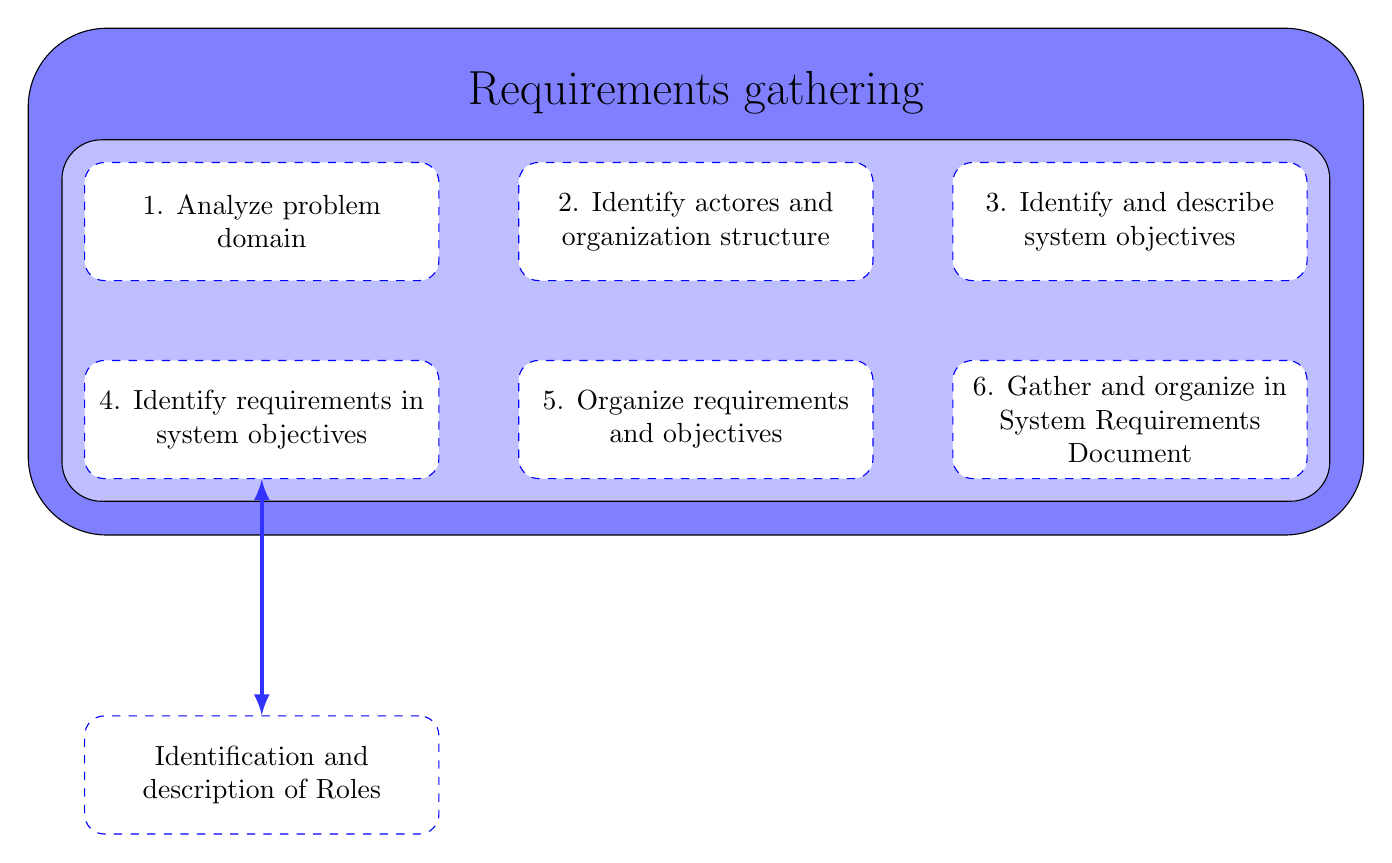
\begin{tikzpicture}
  \node[lvl3] (1) {1. Analyze problem domain};
  \node[lvl3,right=of 1] (2) {2. Identify actores and organization structure}; 
  \node[lvl3,right=of 2] (3) {3. Identify and describe system objectives}; 
  \node[lvl3,below=of 1] (4) {4. Identify requirements in system objectives};
  \node[lvl3,right=of 4] (5) {5. Organize requirements and objectives};
  \node[lvl3,right=of 5] (6) {6. Gather and organize in System Requirements Document};
  \node[lvl2,fit=(1) (2) (3) (4) (5) (6)] (group1) {};
  \node[title,above=0.2cm of group1] (title1) {Requirements gathering};
  \node[lvl1,fit=(title1) (group1)] {};
  \node[lvl3,below=3cm of 4] (roleID) {Identification and description of Roles};
  \draw[myarrow] (roleID.north)--(4.south);
\end{tikzpicture}
\end{document}